\documentclass[10pt]{beamer}
\usepackage{xeCJK}
\usepackage{listings}
\usepackage{tikz}
\usepackage{subfigure}
\usepackage{color}
\usepackage[ruled,linesnumbered,titlenotnumbered,noend,vlined]{algorithm2e}
\usetikzlibrary{arrows,automata}

\renewcommand{\thealgocf}{}

\usetheme[
%	sidebar, % 默认不显示包含幻灯片结构的边框。如设置sidebar选项,则参考AAU模板显示左边框
	footline,
	blue, % 主色调默认为红色,色调可以选择red和blue
%	wide, % 幻灯片的长宽比默认为4:3,如设置了wide选项则为16:9
	hideallsubsections, % 默认显示所有等级的标题。如设置了hideallsubsections,
	                    % 则不显示小节标题
	mathserif, % 默认公式字体是钝化的,如设置mathserif选项则采用正常的公式字体
%	english, % 默认幻灯片环境为中文,如设置english选项则采用英文的章节和图表编号
	sectiontoc, % 设置sectiontoc选项则在每节(section)之前添加一个所有节的目录,
	            % 并标明本节在整个幻灯片中的位置,不建议和\part层级一同使用
]{SEUstyle}

\title[第四组报告]{强化学习与规划 \\ 强化学习在游戏中的应用}
\author[张舒韬 et al.]{刘翔~吴江恒~张舒韬~赵倩隆}
\institute[SEU CS Dept. Team 4]{东南大学\ 计算机科学与工程学院\ 第4组}

\begin{document}
	{\background
		\begin{frame}[plain,noframenumbering]
			\titlepage
		\end{frame}
	}

	\begin{frame}{总目录}
		第I部分 强化学习与规划
		\tableofcontents[part=1]
		第II部分 强化学习在FPS游戏中的应用
		\tableofcontents[part=2]
	\end{frame}

	\part{强化学习与规划}\label{part:rl-and-planning}
	
	\section{背景知识回顾}
	
	\subsection{马尔科夫决策过程}
	
	\begin{frame}{马尔科夫决策过程}{定义}
		\visible<1->{
			一个马尔科夫决策过程是一个五元组$D = \langle S,A,P,r,\gamma \rangle$,其中
			\begin{description}
				\item[$S$] 过程中的状态(state)集合
				\item[$A$] 过程中的动作(action)集合
				\item[$P$] 转移函数(transition function)$P(s, a, s')$定义为$S \times A \times S \rightarrow [0,1]$,表示在状态$s$时选择动作$a$达到状态$s'$的概率
				\item[$r$] 奖励函数(reward function)$r(s, a, s')$定义为$S \times A \times S \rightarrow \mathbb{R}$,表示在状态$s$时选择动作$a$达到状态$s'$时得到的奖励
				\item[$\gamma$] 折扣因子(discount factor)$\gamma \in [0,1]$
			\end{description}
		}
		
		\visible<2->{
			累积奖励的定义
			\begin{equation*}
			\sum^{\infty}_{t=0} {\gamma^t r(s_t, a_t, s_{t+1})}   
			\end{equation*}
		}
	\end{frame}

	\begin{frame}{马尔科夫决策过程}{问题}
		\begin{description}
			\item<2->[预测问题(Predicting)] 已知起始状态、转移函数和决策策略,求在此情况下能够得到的累积奖励的期望;
			\item<3->[规划问题(Planning)] 已知起始状态和转移函数,求使累积奖励的期望值最大的决策策略;
			\item<4->[强化学习(Reinforcement Learning)] 转移函数或奖励函数未知,求使累积奖励的期望值最大的决策策略。
		\end{description}
	\end{frame}

	\begin{frame}{马尔科夫决策过程}{规划与学习}
		\begin{figure}
			\centering
			\begin{tikzpicture}[->,>=stealth',shorten >=1pt,auto,node distance=30cm,semithick,bend angle=40]
			\tikzstyle{every state}=[rectangle,font=\bfseries,fill=white,draw=none,text=black]
			\node (policy) at (0,0)           [state] {value/policy};
			\node (exper)  at (1*2,-1.732*2)  [state] {experience};
			\visible<1,3>{\node (model)  at (-1*2,-1.732*2) [state] {model};}
			
			\path (policy) edge [bend left] node {acting} (exper);
			\visible<1-2>{\path (exper)  edge [bend left] node {direct RL} (policy);}
			\visible<1,3>{\path (exper) edge [bend left] node {model learning} (model);}
			\visible<1,3>{\path (model)  edge [bend left] node {planning} (policy);}
			
			\only<1>{\node at (0,-5.5) [state] { };}
			\only<2>{\node at (0,-5.5) [state,text=red] {Model-Free RL};}
			\only<3>{\node at (0,-5.5) [state,text=red] {Model-Based RL};}
			\end{tikzpicture}
			\caption{学习、规划和执行之间的关系\protect\cite{Sutton1998:RL-Introduction}}\label{fig:relation-in-RL}
		\end{figure}
	\end{frame}

	\subsection{Q-Learning}
	
	\begin{frame}{Q-Learning}{定义}
		\begin{itemize}
			\item<2-> Q-Learning是一种off-policy的时序差分学习方法
			\item<3-> Q-Learning的目标是得到$Q^*$函数的估计,即
			\[Q^*(s,a) = \max_{\pi}\mathbb{E}(R_t | s_t = t, a_t = a, \pi) \]
			\[Q^*(s,a) = \mathbb{E}\left[r_{t+1} + \gamma \max_{a' \in A(s)} Q^*(s_{t+1}, a') | s_t = s, a_t = a\right] \]
			\item<4-> Q-learning的定义为
			\[ Q(s_t, a_t) \gets Q(s_t, a_t) + \alpha \left[r_{t+1} + \gamma \max_{a \in A(s_{t+1})}Q(s_{t+1}, a) - Q(s_t, a_t) \right] \]
		\end{itemize}
	\end{frame}

	\begin{frame}{Q-Learning}{算法描述}
		\begin{algorithm}[H]
			随机初始化$Q(s, a)$\;
			\ForEach{每个周期(episode)}{
				初始化$s$\;
				\ForEach{周期内的每一步,直到$s$为终止状态}{
					利用$Q$函数中获得的策略(例如$\epsilon$-greedy)选择状态$s$时采取的策略\;
					执行$a$,观察$s'$和$r'$\;
					$Q(s_t, a_t) \gets Q(s_t, a_t) + \alpha [r_{t+1} + \gamma \max_{a}Q(s_{t+1}, a) - Q(s_t, a_t) ]$\;
				}
			}
			\caption{Q-Learning}\label{alg:q-learning}
		\end{algorithm}
	\end{frame}

	\begin{frame}{基于强化学习的规划}{Q-Planning}
		
		\begin{figure}
			\centering
			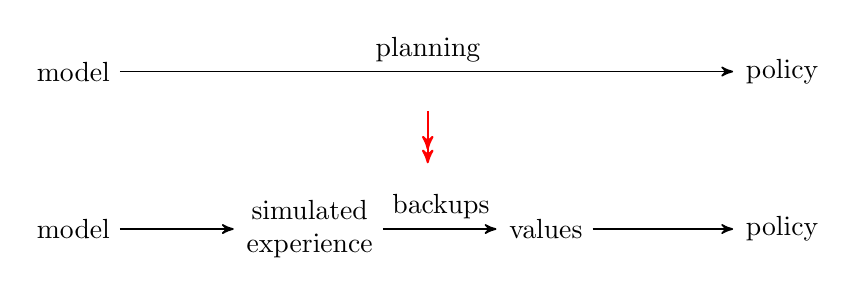
\begin{tikzpicture}[->,>=stealth',shorten >=1pt,auto,node distance=50cm,semithick]
			\tikzstyle{every state}=[rectangle,fill=white,draw=none,text=black,align=center]
				\visible<2->{
					\node (model0) at(0,2) [state] {model};
					\node (policy0) at(9,2) [state] {policy};
					
					\path (model0) edge node {planning} (policy0);
				}
			
				\visible<3-> {
					\draw [->>,thick,draw=red] (4.5,1.5) -- (4.5,0.8);
					\node (model) at(0,0) [state] {model};
					\node (exper) at(3,0) [state] {simulated\\ experience};
					\node (values) at(6,0) [state] {values};
					\node (policy) at(9,0) [state] {policy};
					
					\path (model) edge (exper)
					(exper) edge node {backups} (values)
					(values) edge (policy);
				}
			\end{tikzpicture}
		\end{figure}
	
		\visible<4->{
			\begin{algorithm}[H]
				\Repeat{stop}{
					随机选择$s \in S$, $a \in A(s)$\;
					根据模型模拟出下一状态$s'$和奖励$r$\;
					更新$Q(s,a) \gets Q(s,a) + \alpha[r + \gamma \max_{a'}Q(s',a') - Q(s,a)]$\;
				}
				\caption{随机Q-Planning}
			\end{algorithm}
		}
		
	\end{frame}

	\begin{frame}{强化学习}{强化学习的两种方法}
		\begin{small}		
			\begin{description}
				\item<2->[Model-Based RL] 
				
				优点:
				\begin{itemize}
					\item 有时直接从环境中学到值函数较难,而模型的$P(s’|s,a)$和$R(r|s,a)$很容易就能用监督学习去学;
				\end{itemize}
				
				缺点:
				\begin{itemize}
					\item 误差来源多了模型拟合的误差;
				\end{itemize}
				
				\item<3->[Model-Free RL] 优点:
				\begin{itemize}
					\item 不需要具体的环境模型;
					\item 使用时做出决策的时间快;
				\end{itemize}
				
				缺点:
				\begin{itemize}
					\item 优化过程可能不稳定且不收敛;
					\item 比较难适应变化的环境;
				\end{itemize}
			\end{description}
		\end{small}
	\end{frame}

	\begin{frame}{强化学习}{Model-Free or Model-Based?}
		All models are wrong, but some are useful.
		\begin{flushright}
			--George E.P. Box, Robustness in the strategy of scientific model building
		\end{flushright}
	
		\begin{figure}
			\centering
			\begin{tikzpicture}
				\visible<2->{\node at (0,0) {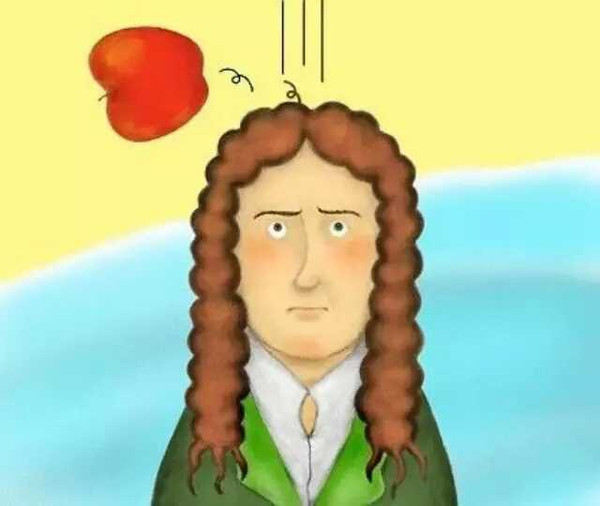
\includegraphics[width=.4\linewidth]{pictures/newton.png}};}
				\visible<3->{\node at(2,0) {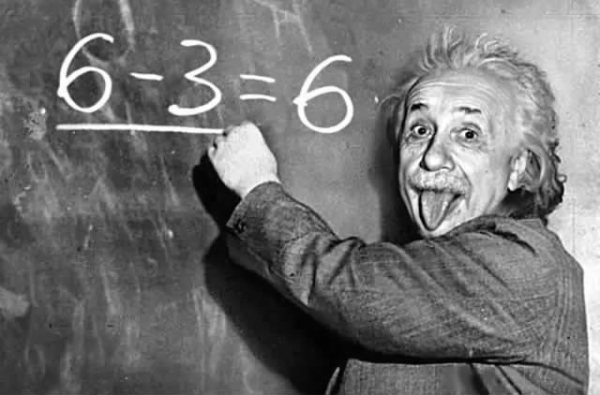
\includegraphics[width=.5\linewidth]{pictures/einstein.png}};}
				\visible<4->{\node at(4,0) {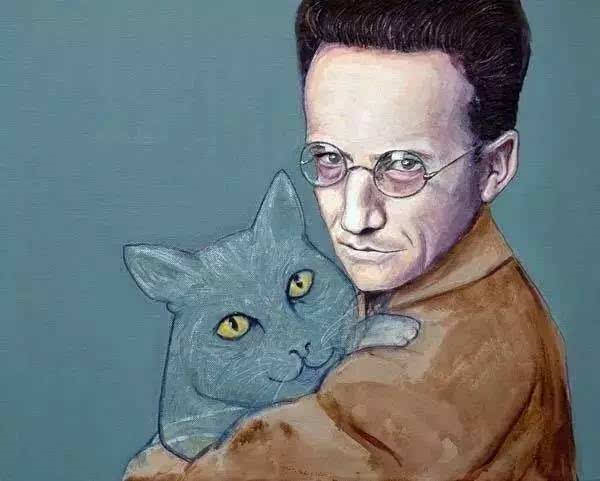
\includegraphics[width=.4\linewidth]{pictures/cat.png}};}
			\end{tikzpicture}
		\end{figure}
	\end{frame}

	\section{两种规划与学习结合的方法}
	
	\subsection{Dyna}
	
	\begin{frame}{Dyna}{主要思想和结构}
		\begin{figure}
			\centering
			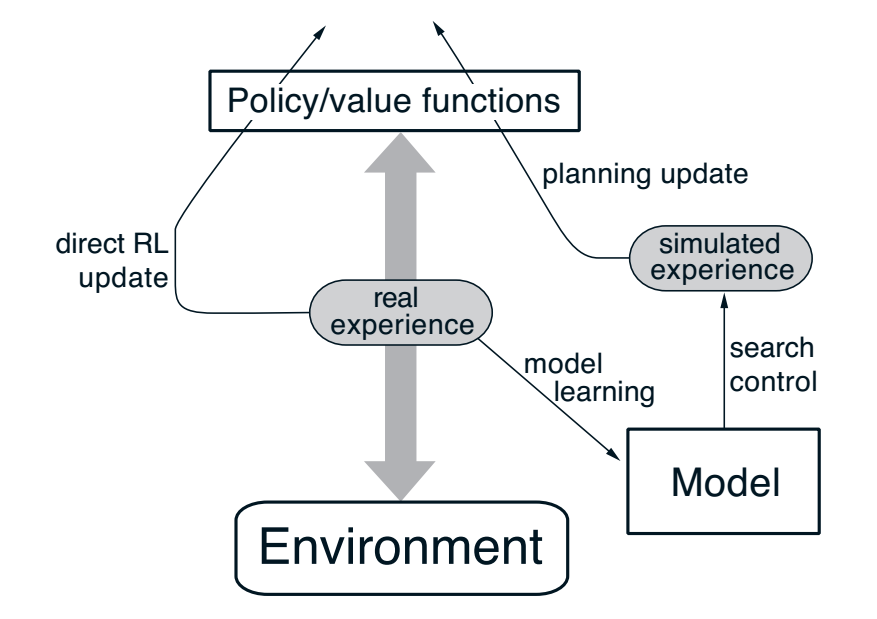
\includegraphics[width=0.6\linewidth]{pictures/dyna-arch.png}
			\caption{Dyna agent的一般结构}
			\label{fig:dyna-arch}
		\end{figure}
		
		\begin{itemize}
			\item<2-> Dyna\cite{Sutton1990:Dyna}包括了图\ref{fig:relation-in-RL}中的所有过程,即\alert{规划}、\alert{执行}、\alert{模型学习}和\alert{值函数学习}
			\item<3-> 规划时使用一个确定的模型(即$P(s,a,s') \rightarrow \{0,1\}$),该模型在;执行过程中不断更新;
		\end{itemize}
	\end{frame}

	\begin{frame}{Dyna}{Dyna-Q}
		\begin{algorithm}[H]
			对任意的$s \in S$,$a \in A(s)$,初始化$Q(s,a)$和$Model(s,a)$\;
			\Repeat{stop}{
				对当前状态$s$,根据$Q$表选择$a \in A(s)$并执行,得$s'$和$r$\;
				更新$Q(s,a)$\;
				\textcolor{blue}{用$s',r$更新$Model(s,a)$\;}
				\alert{
				\Repeat(\tcp*[f]{在$Model$上规划并更新$Q$}){$N$次循环}{
					$s$为任意观察到的状态,$a$为$s$上进行过的任意操作\;
					$s',r \gets Model(s,a)$\;
					$Q(s,a) \gets Q(s,a) + \alpha [r + \gamma\max_{a'}Q(s',a') - Q(s,a)]$\;
				}}
			}
			\caption{Dyna-Q算法}\label{alg:dyna-q}
		\end{algorithm}
	\end{frame}

	\begin{frame}{Dyna}{实验}
		\begin{figure}
			\centering
			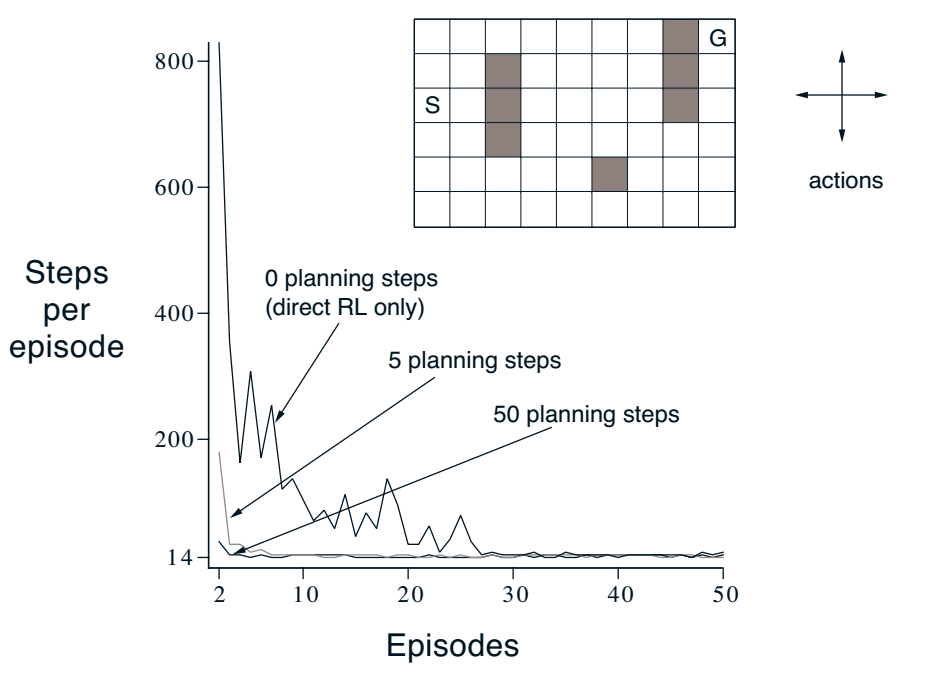
\includegraphics[width=0.7\linewidth]{pictures/dyna-exp}
			\caption[Dnya-Q 迷宫]{Dyna-Q在一个迷宫问题上的实验,agent需要从S走到G,$r\rightarrow \{0,1\}$。对于所有的$N$,第一次探索是一样的,都是大约1700步;之后,Dyna-Q和Q-Learning的差别开始显现}
			\label{fig:dyna-exp}
		\end{figure}
	\end{frame}

	\begin{frame}{Dyna}{错误的模型-原因}
		模型出错的原因:
		\begin{itemize}
			\item 先验知识存在错误
			\item 随机环境难以用模型描述或估计
			\item 环境出现变化
		\end{itemize}
		
		处理方法:学习过程中不断使用从环境中获得的数据对模型进行更新和纠正
	\end{frame}
	
	\begin{frame}{Dyna}{错误的模型-实验}
		\begin{figure}
			\centering
			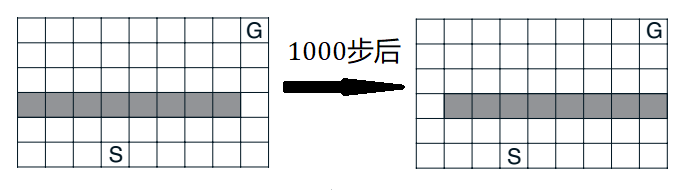
\includegraphics[width=0.5\linewidth]{pictures/blocking-maze}
			\caption{1000步之后,迷宫出现变化,左侧墙壁打开,右侧通路封闭}
			\label{fig:blocking-maze}
		\end{figure}
		
		\visible<2->{
			\begin{figure}
				\centering
				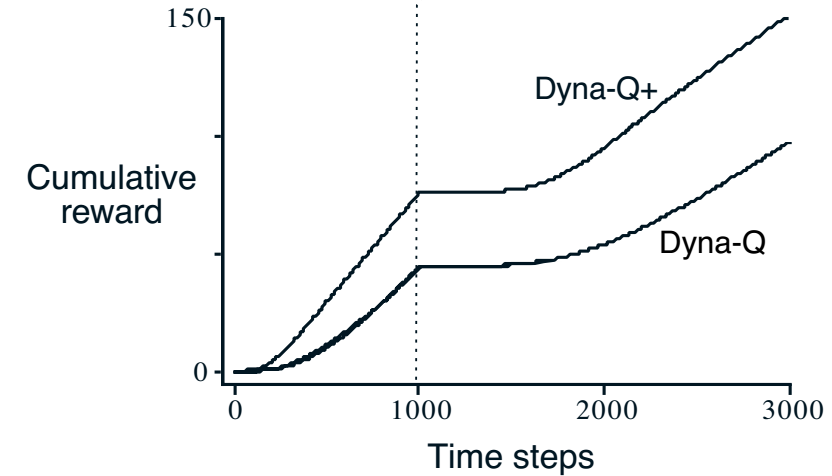
\includegraphics[width=0.5\linewidth]{pictures/blocking-maze-result}
				\caption{由于Dyna算法包括了对模型的更新,agent在一段时间后完成了对环境的重新建模并找到了正确的路径。图中Q+是加强了探索能力的Q-Learning,用$r+\kappa \sqrt{n}$为奖励函数,$n$为$s$状态下$a$连续未被选中的次数}
				\label{fig:blocking-maze-result}
			\end{figure}
		}
	\end{frame}
	
	\subsection{DARLING}
	
	\begin{frame}{DARLING}{方法介绍}
		DARLING方法\cite{Leonetti2016:AutoPlan-RL}的求解步骤:
		\begin{enumerate}
			\item<2-> 根据预设的模型,用规划求解器(例如ASP推理机)求解某个度量值(例如规划的步骤数量)在阈值内的规划方案;
			\item<3-> 筛选合并求得的规划方案,删除包含冗余步骤的方案,融合后得到部分策略,即在各个状态下可选的行动集合;
			\item<4-> 执行和学习,在执行中仅选择部分策略中的行为,学习它们的累积奖励的期望并优化策略。
		\end{enumerate}
	
	\end{frame}

	\begin{frame}{DARLING}{建模,规划,筛选,合并}
		\begin{description}
			\item<2->[建模(Modeling)] 对环境$D=\langle S, A, P, r,\gamma \rangle$进行建模,建立从环境状态到模型状态的函数$o:S \rightarrow S_m$,得$D_m = \langle S_m, A, P_m \rangle$,其中
			\item<3->[规划(Planning)] 利用规划工具,以一定的冗余度计算可行的方案。规划是在一个假设的模型上执行的,因此不能保证所得的方案是最优甚至可行的;
			\item<4->[筛选(Filtering)] 如果规划方案中存在重复出现的状态和动作(例如存在环),则认为方案是冗余的,可以被更短的方案代替;
			\item<5->[合并(Merging)] 合并筛选过的方案,得到可达状态和这些状态下可选择的动作的集合,即一个简化的模型$D_r$;
		\end{description}
		
		\vspace{10pt}
		\visible<5->{
			从Planning到Merging的过程其实是将假设中的模型$D_m$做了进一步的化简和压缩。
		}
	\end{frame}

	\begin{frame}{DARLING}{Planning \& Filtering and Merging-例}
		\begin{figure}
			\centering
			\subfigure[迷宫问题,要求机器人从S走到G,图中红色横线为一扇可能开启或关闭的门。Planning步骤求长度小于最短方案的1.5倍的方案]{
			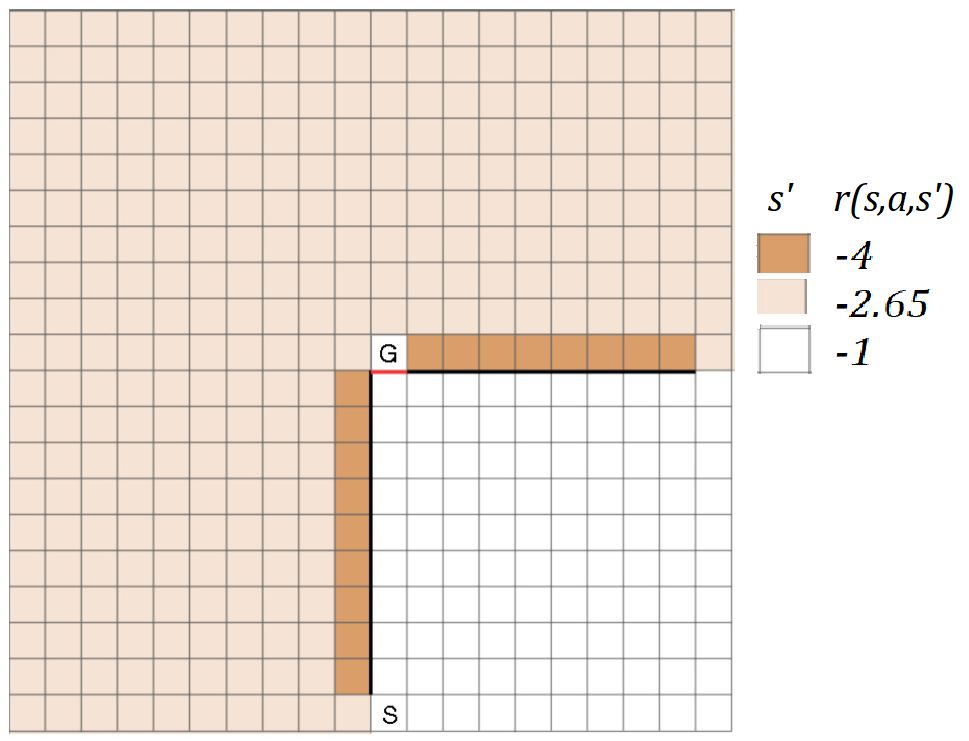
\includegraphics[width=0.475\linewidth]{pictures/grid-world.png}
			}
			\subfigure[部分策略,由筛选后的non-redudant方案融合而成]{
			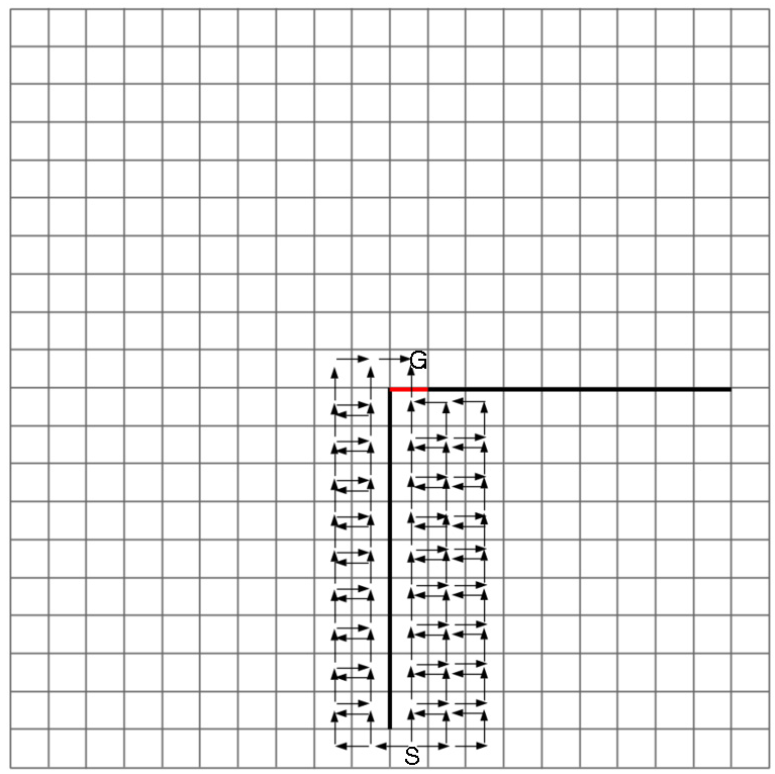
\includegraphics[width=.35\linewidth]{pictures/partial-policy.png}
			}
			\label{fig:grid-world}
		\end{figure}
	
	\end{frame}

	\begin{frame}{DARLING}{Execution and learning}
		\begin{itemize}
		\item 实际的转移函数和模型中设想的转移函数并不一致。这会导致agent在执行和学习的过程中进入了模型中没有的状态。此时应该以新出现的状态为初始状态,重新进行规划,并将所得的部分策略添加到已有的部分策略中;
		
		\item 在所得模型上的RL与其他的强化学习并无太大差别,任意的强化学习方法都可以实现。
		\end{itemize}
	\end{frame}

	\begin{frame}{DARLING}{实验}
		\begin{itemize}
			\item<2-> 实验采用的环境如图\ref{fig:grid-world}所示。仅在agent到达门口时才获知门是否打开(Partial Observed MDP,POMDP),在周期$e$时门打开的概率为
				\[p(e)=
					\begin{cases}
						1 - \frac{e}{E-1} & 0 \leq e < E \\
						0 & \text{other wise}
					\end{cases}
				\]
			\item<3-> 实验中用到了以下几种agent:
			\begin{description}
				\item[P agent]<4-> 仅在$D_m$上进行规划;
				\item[RL agent]<5-> 仅在$D$上进行强化学习;
				\item[PRL agent]<6-> 采用DARLING方法,在$D_m$上计算部分策略,并将强化学习的探索限制在$D_r$上;
				\item[Pmem-n agent]<7-> 采用DARLING方法,有前$n$个周期内观察门是否打开的记忆,并以此估计当前门是否打开;
			\end{description}
		\end{itemize}
	\end{frame}

	\begin{frame}{DARLING}{实验结果}
		\begin{figure}
			\centering
			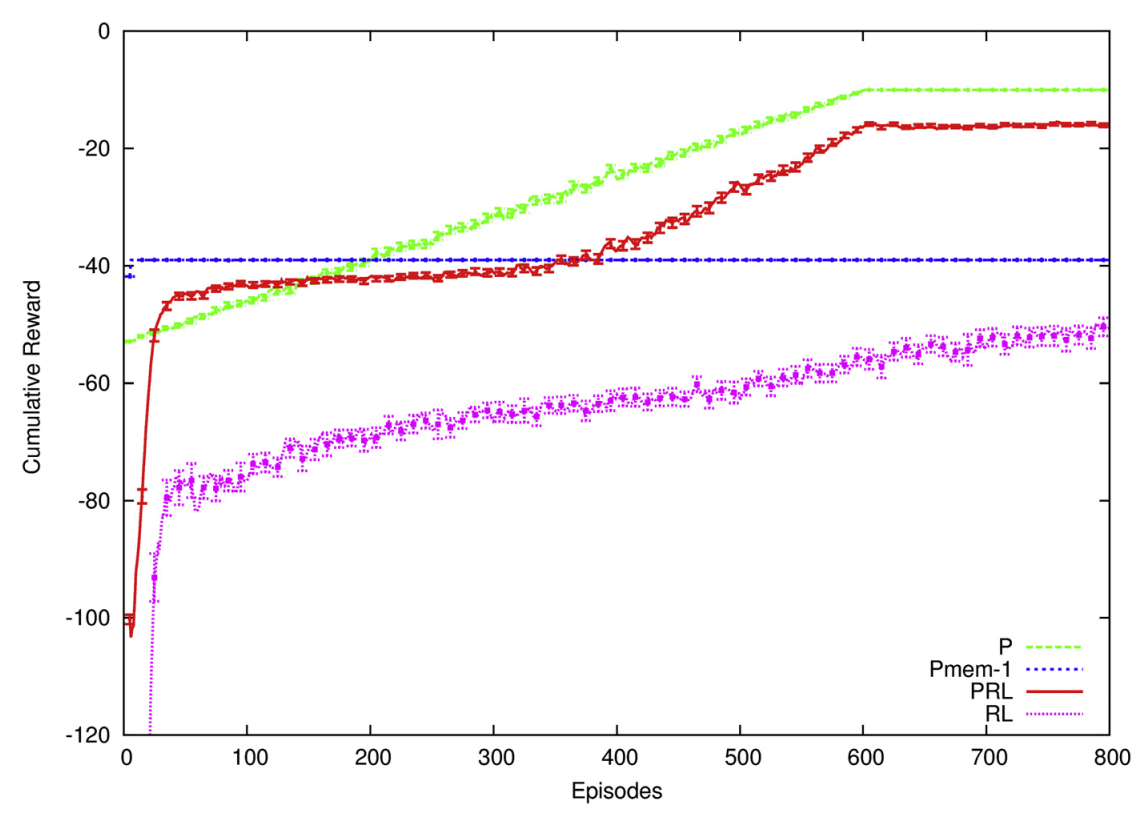
\includegraphics[width=0.6\linewidth]{pictures/darling-expr}
			\caption{实验结果}
			\label{fig:darling-expr}
		\end{figure}
		\visible<2->{
			\only<2>{P agent的累积奖励变化与$p(e)$的概率保持一致。但由于实际应用中,$D_m$和$D$差距较大,因此直接使用规划方法不可能取得如此良好的结果。}
			\only<3>{RL agent很快学到了最优策略,但环境变化后没有能发现更优的策略。}
			\only<4>{PRL agent学到了最优策略,并在环境变化后选择了更优的策略。}
			\only<5>{Pmem-n agent被起初的观察限制,没有发现环境的变化,因此没有发现更优的策略。实际上,无论$n$的取值如何,agent在不稳定的环境中都没有获得最优策略。}
		}
	\end{frame}

	\section{事后经验回放与稀疏奖励下的规划}
		
	\part{强化学习在游戏中的应用}\label{part:rl-in-fps}
	
	\section{Atari游戏与DQN}
	
	\part{FPS游戏与DRQN}
	
	\section{DRQN}
	
	\begin{frame}{Deep Q-Network 回顾}
		\begin{columns}
			\begin{column}{.6\linewidth}
				\begin{itemize}
					\item 前面提到,DQN在Atari游戏中,有能力学习到不输人类的控制策略。
					\item 它仅仅将游戏最近4帧的原始画面作为输入,就使agent在Atari游戏中有了能与人类相抗衡的表现。
					\item 但是,DQN在需要记忆\alert{超过最近4帧}画面的游戏中表现不佳,这类游戏未来的state和reward不仅依赖于当前输入的画面,还依赖于更早画面中的信息。
					\item 上述现象是一种 Partially-Observable Markov Decision Process (POMDP)。
				\end{itemize}
			\end{column}
			\begin{column}{.4\linewidth}
				\begin{figure}
					\centering
					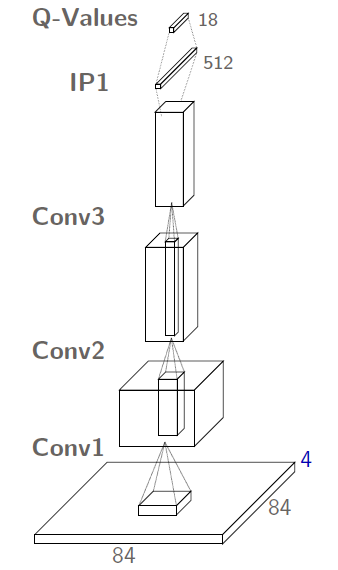
\includegraphics[width=0.9\linewidth]{pictures/dqn-architecture-2}
					\caption{}
					\label{fig:dqn-architecture-2}
				\end{figure}
				
			\end{column}
		\end{columns}
		
	\end{frame}

	\begin{frame}{从DQN到DRQN}
		为解决前述POMDP问题,我们需要对原始的DQN加以改进,Deep Recurrent Q-Network应运而生。
		\begin{columns}[c]
			\begin{column}{.4\linewidth}
				\begin{figure}
					\centering
					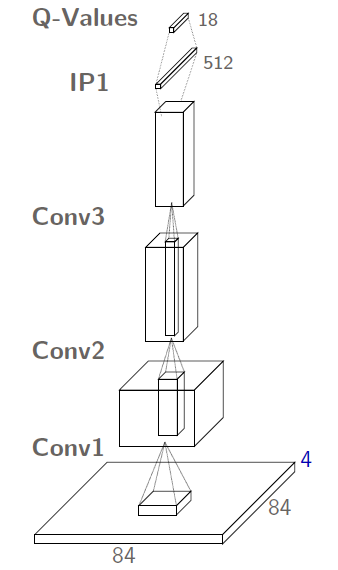
\includegraphics[width=0.9\linewidth]{pictures/dqn-architecture-2}
				\end{figure}
			\end{column}
			\begin{column}{.1\linewidth}
				\begin{figure}
					\centering
					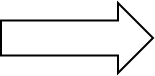
\includegraphics[width=0.9\linewidth]{pictures/big-arrow}
				\end{figure}
			\end{column}
			\begin{column}{.5\linewidth}
				\begin{figure}
					\centering
					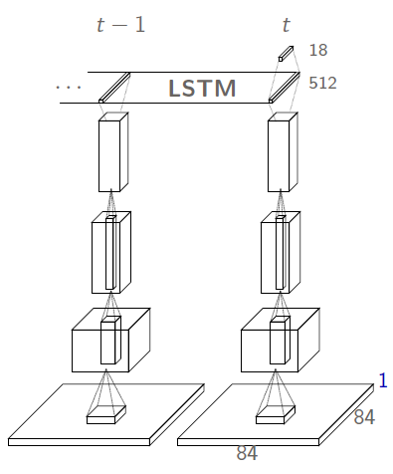
\includegraphics[width=0.9\linewidth]{pictures/drqn-architecture}
				\end{figure}
				
			\end{column}
		\end{columns}
	\end{frame}

	\begin{frame}{Deep Recurrent Q-Network}
		\begin{columns}
			\begin{column}{.6\linewidth}
				与DQN相比,DRQN:
				\begin{itemize}
					\item 将原本的全连接层替换为相同维度的Long-Short Term Memory (LSTM).
					
					\item 每一个timestep只接受一帧画面作为输入。
					
					\item LSTM为过去的状态提供记忆能力。
					
				\end{itemize}
			\end{column}
			\begin{column}{.4\linewidth}
				\begin{figure}
					\centering
					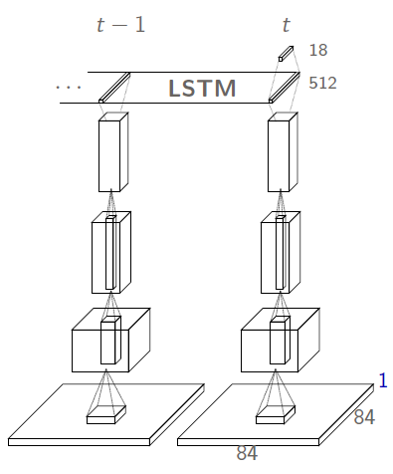
\includegraphics[width=0.9\linewidth]{pictures/drqn-architecture}
					\caption{}
					\label{fig:drqn-architecture}
				\end{figure}
				
			\end{column}
		\end{columns}
	\end{frame}

	\begin{frame}{Research Line}
		\begin{itemize}
			\item Intelligent decision making is the heart of AI.
			
			\item Desire agents capable of learning to act intelligently in diverse environments.
			
			\item Reinforcement learning provides a general learning framework.
			
			\item RL + deep neural networks yields robust controllers that learn from pixels. (DQN)
			
			\item DQN lacks mechanisms for handling partial observability.
			
			\item Extend DQN to handle Partially Observable Markov Decision Processes (POMDPs).
			
		\end{itemize}
	\end{frame}

	\begin{frame}{DRQN}{实验:DRQN vs DQN}
		\begin{itemize}
			\item 比较对象:
				\begin{itemize}
					\item DRQN;
					\item 扩展DQN(将普通DQN的输入扩展到10张图片);
					\item DQN.
				\end{itemize}
			
			\item 实验目标:
				\begin{itemize}
					\item Standard Atari games
					\item Flickering Atari games
				\end{itemize}
			
		\end{itemize}
	\end{frame}

	\begin{frame}{DRQN vs DQN}{实验结果}
		\begin{figure}
			\centering
			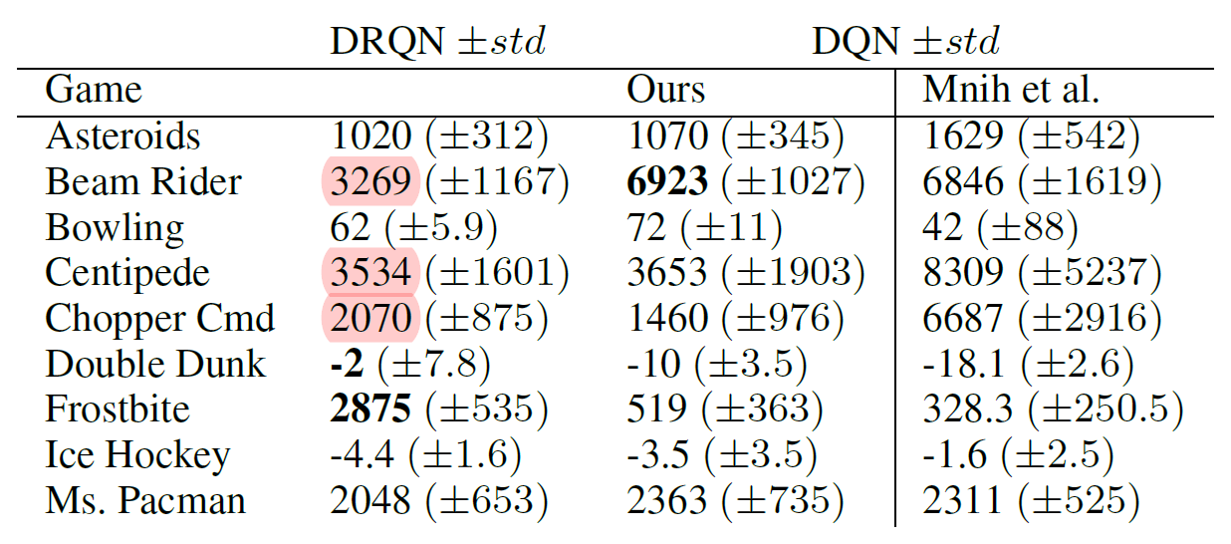
\includegraphics[width=0.9\linewidth]{pictures/dqn-vs-drqn-result}
			\caption{DRQN的表现勉强达到DQN的水平}
			\label{fig:dqn-vs-drqn-result}
		\end{figure}
		
	\end{frame}

	\begin{frame}{DRQN}{Flickering Atari games}
		\begin{columns}
			\begin{column}{.6\linewidth}
				以一个随机概率遮蔽屏幕,使游戏呈现partially observability.
				%这个公式是哪里来的?
				\[o_t
					\begin{cases}
						s_t & with p = \frac{1}{2} \\
						\langle 0, \dots, 0 \rangle & \text{otherwise}
					\end{cases}
				\]
				
				现在,当前的游戏状态只能够从历史状态中获取到了。
			\end{column}
		
			\begin{column}{.4\linewidth}
				\begin{figure}
					\centering
					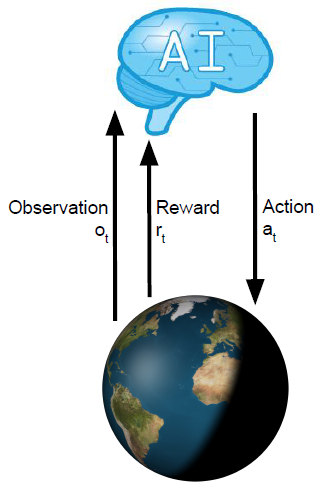
\includegraphics[width=0.7\linewidth]{pictures/pomdp}
				\end{figure}
			\end{column}
		\end{columns}
	\end{frame}

	\begin{frame}{DRQN}{Results: Flickering Atari games}
		\begin{figure}
			\centering
			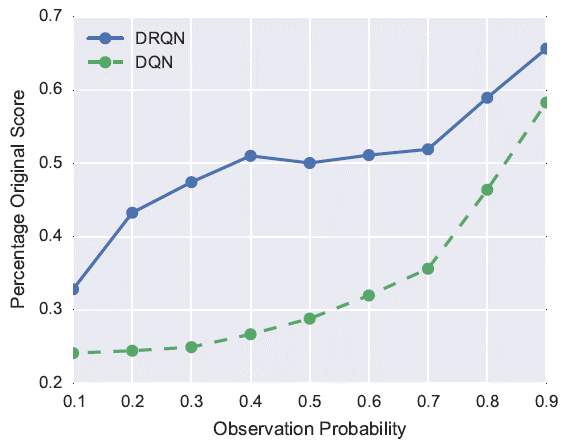
\includegraphics[width=0.7\linewidth]{pictures/flickering-atari-result}
			\caption{横轴:某时间步能够观测到游戏画面的概率;纵轴:各模型与自己Standard Atari games得分的比值}
			\label{fig:flickering-atari-result}
		\end{figure}
		
	\end{frame}

	\begin{frame}{DRQN}{结论}
		\begin{itemize}
				\item 在Standard Atari games中,DRQN的表现勉强比上DQN
				\item 在Flickering Atari game中,DRQN表现下降的幅度比DQN小得多
		\end{itemize}
	
		\visible<2->{但这样的结果远远不能让人满意……}
	\end{frame}
	
	\section{用DRQN玩FPS游戏}

	\begin{frame}{DRQN for FPS}{}
		FPS即第一人称射击游戏(First person shooting games),与Atari 2600相比,FPS游戏具有以下特点:
	
		\begin{itemize}
			\item 操作更加复杂,行为更加丰富(搜索地图,收集道具,识别并打败敌人…);
			\item 画面只能观测到部分游戏状态(partially observable);
			\item FPS与现实场景相似,相关技术适合在机器人开发中得到应用。
		\end{itemize}
	\end{frame}

	\begin{frame}{DRQN for FPS}{VizDoom}
		VizDoom是一个基于Doom的AI研究平台,主要针对面向原始视觉信息输入的增强学习。
		
		Doom Deathmatch规则介绍:
		http://vizdoom.cs.put.edu.pl/
		
		\begin{figure}
			\centering
			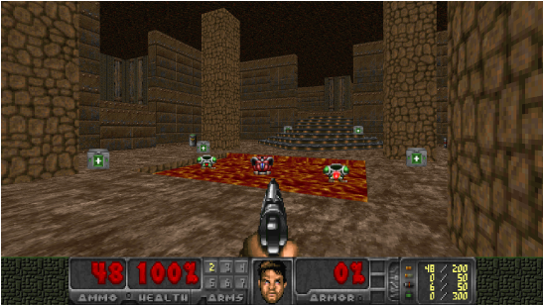
\includegraphics[width=0.8\linewidth]{pictures/deathmatch}
		\end{figure}
	\end{frame}

	\begin{frame}{DRQN for FPS}{Baseline DRQN model}
		首先,直接利用原始的DRQN运用在ViZDoom上,效果并不好。
		\begin{itemize}
			\item 训练出的agent会随意开火;
			\item 对使用弹药加以惩罚:如果惩罚过重,agent就不会开火;过轻,agent依然会随意开火。
			\item agent不能够准确地探测敌人
		\end{itemize}
		
	\end{frame}

	\begin{frame}{DRQN for FPS}{Methods}
		\begin{description}
			\item[DRQN augmented with game features] 
			使用了一个增加游戏信息(game features)的DRQN模型来提升性能。
			
			\item[Divide and conquer]
			将游戏过程分为两个阶段分别训练,提升性能并加快了训练速度。
			
		\end{description}
	\end{frame}

	\begin{frame}{Methods}{DRQN augmented with game features-I}
		\begin{figure}
			\centering
			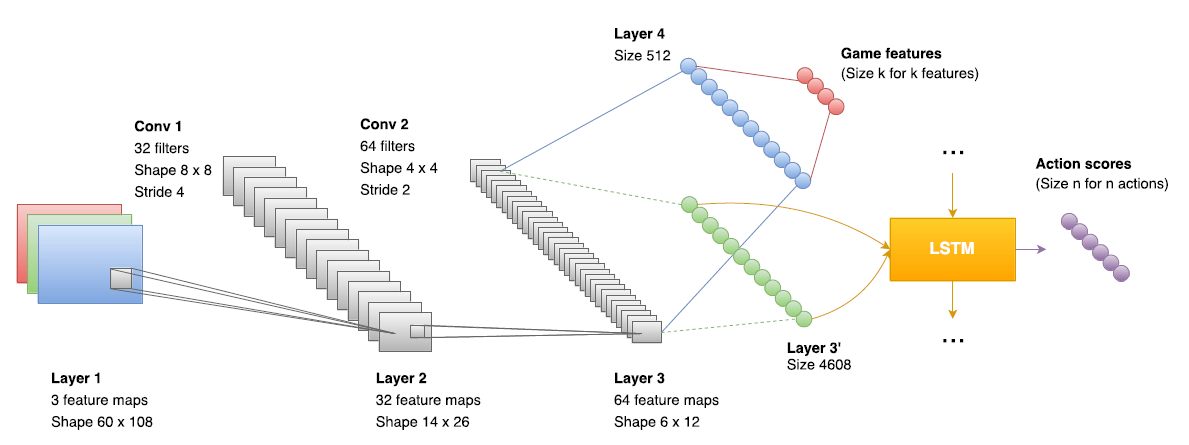
\includegraphics[width=0.7\linewidth]{pictures/drqn-with-game-features}
		\end{figure}
		
	\end{frame}

	\begin{frame}{Methods}{DRQN augmented with game features-II}
		\begin{itemize}
			\item 训练时加入了当前画面的游戏状态信息作为输入;
			
			\item 网络的损失函数是DRQN的损失函数合并上交叉熵损失(cross-entropy loss),同时训练DRQN和游戏状态信息的侦测,使卷积层也能够捕捉到与游戏相关的信息;
			
			\item 虽然可以获得许多游戏信息,但仅考虑画面中是否有敌人的信息,就能使模型的表现有显著的改进。
		\end{itemize}
	\end{frame}

	\begin{frame}{Methods}{With vs without game features}
		\begin{figure}
			\centering
			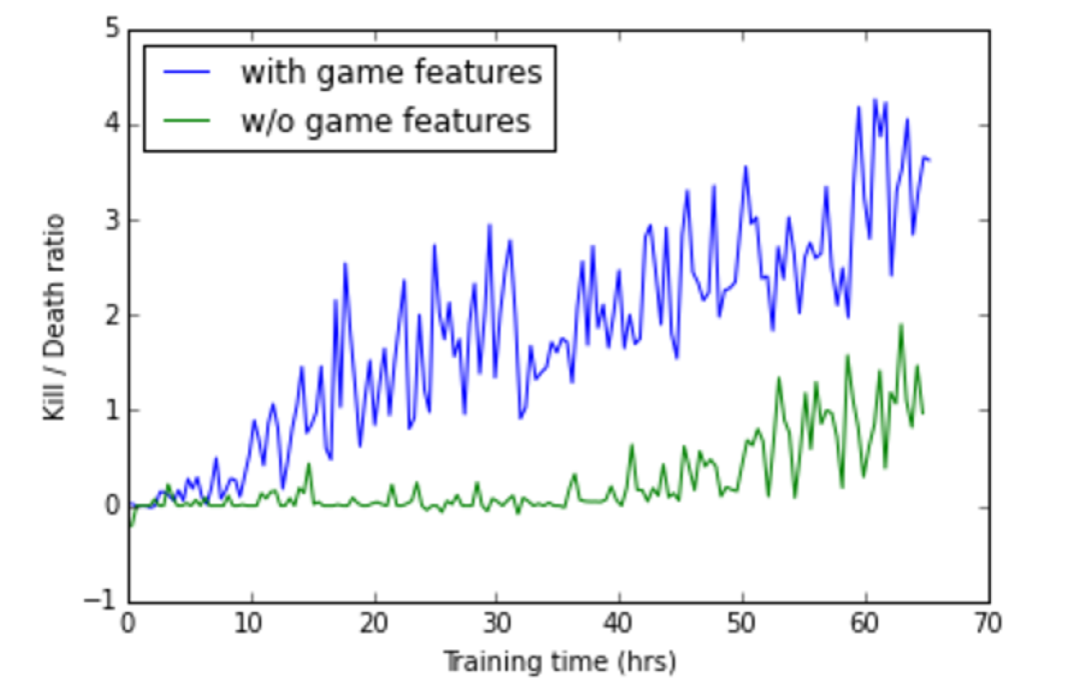
\includegraphics[width=0.7\linewidth]{pictures/with-game-features-result}
			\caption{横轴:训练时间;纵轴:击杀死亡比}
			\label{fig:with-game-features-result}
		\end{figure}
	\end{frame}

	\begin{frame}{Methods}{Divide and conquer-阶段划分}
		Doom Deathmatch 游戏过程被分成两个阶段:导航阶段和行动阶段
		\begin{description}
			\item[导航阶段(the navigation)]  探索地图,收集,发现敌人
			\item[行动阶段(the action)]:攻击敌人
		\end{description}
		
		\visible<2->{	
			当前游戏过程处何阶段由画面中是否有敌人来决定(game feature)。
		}
	
	\end{frame}

	\begin{frame}{Methods}{Divide and conquer-阶段示例}
		\begin{columns}
			\begin{column}{.5\linewidth}
				\begin{figure}
					\centering
					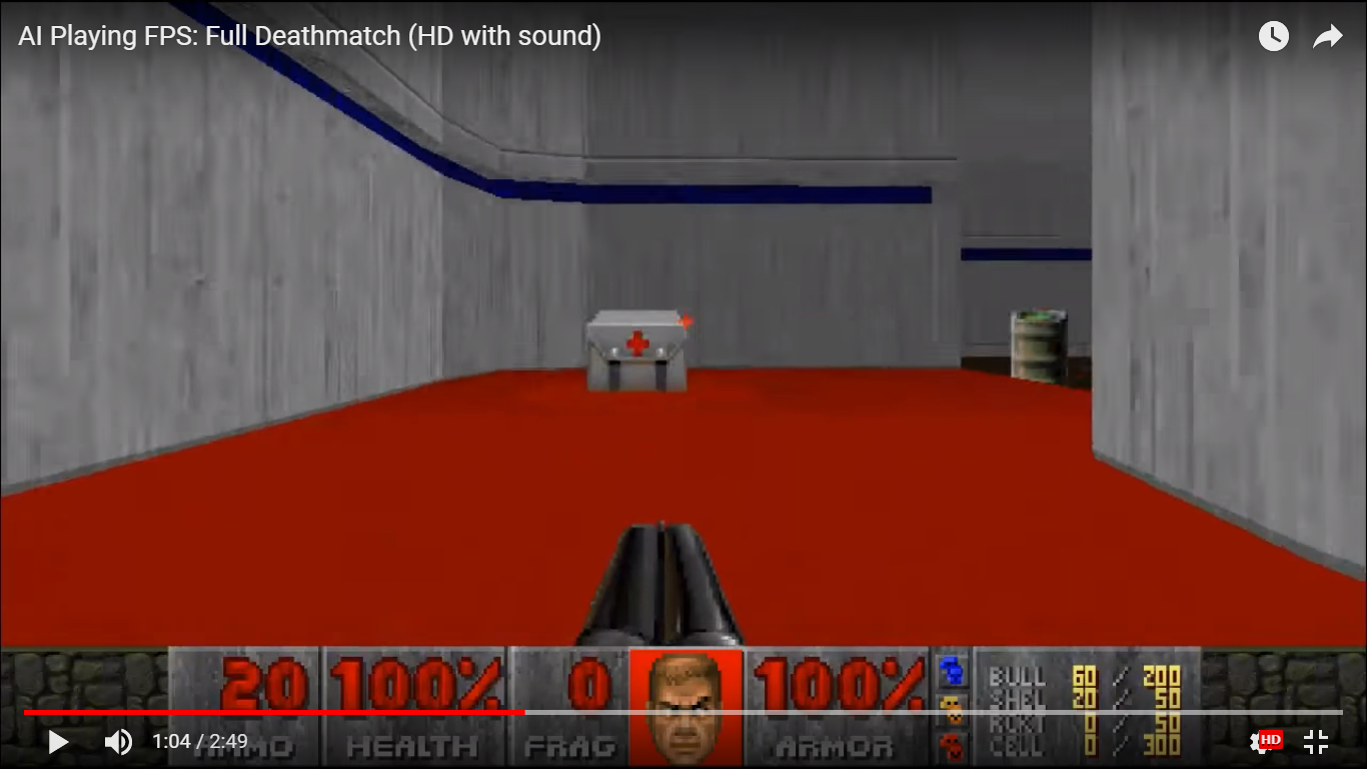
\includegraphics[width=0.9\linewidth]{pictures/deathmatch-2}
					\caption{导航阶段}
					\label{fig:deathmatch-2}
				\end{figure}
			\end{column}
			\begin{column}{.5\linewidth}
				\begin{figure}
					\centering
					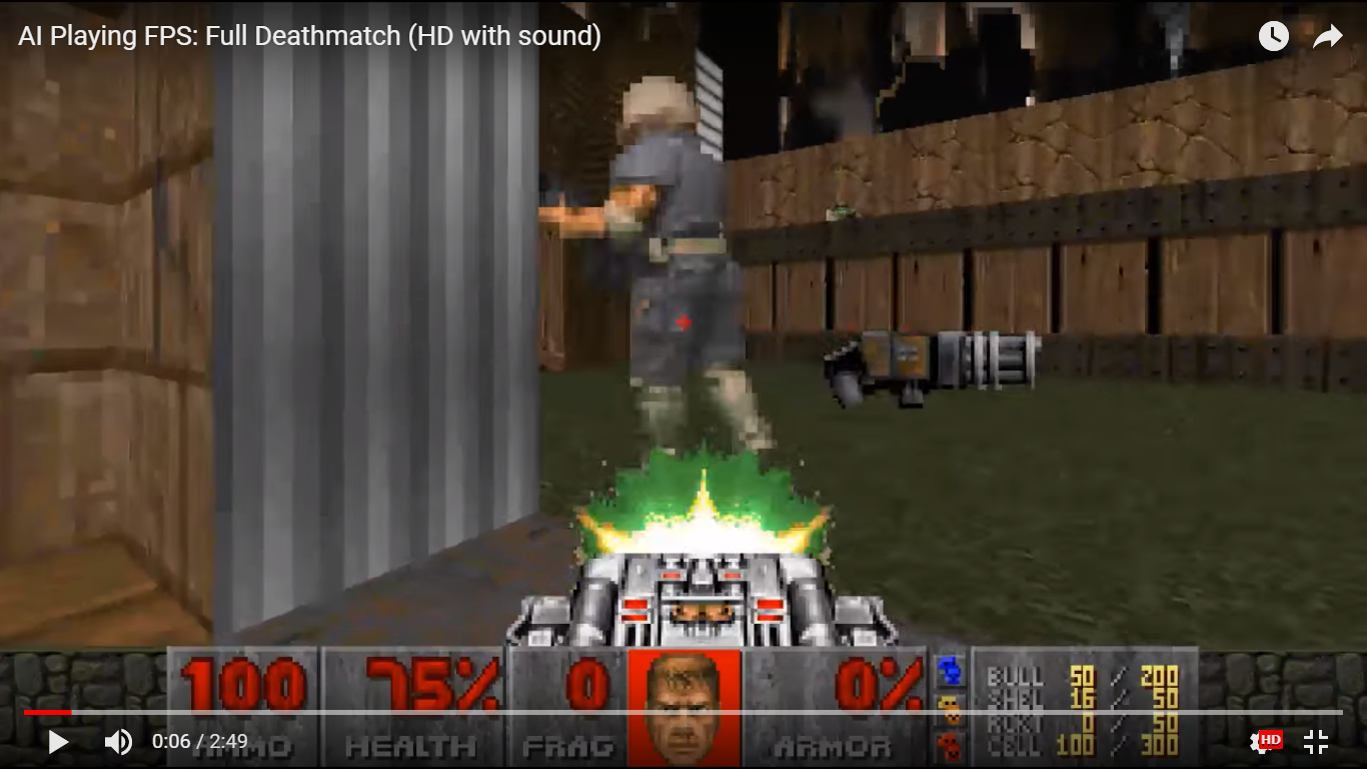
\includegraphics[width=0.9\linewidth]{pictures/deathmatch-3}
					\caption{行动阶段}
					\label{fig:deathmatch-3}
				\end{figure}
				
			\end{column}
		\end{columns}
	\end{frame}

	\begin{frame}{Methods}{Divide and conquer-训练模型}
		对不同的阶段,使用了不同的模型进行训练:
		\begin{description}
			\item[导航阶段] DQN
			\item[行动阶段] DRQN with game features
		\end{description}
		
		\visible<2->{
			目前,DQN并不支持结合多个网络来优化不同的目标,但当前的游戏信息可以由改进的DRQN进行侦测。
		}
		
	\end{frame}

	\begin{frame}{Methods}{Divide and conquer-优点}
		这样的分治策略带来许多优点:
		\begin{itemize}
			\item<2-> 两个网络可以并行训练,大大加快了模型训练速度。
			\item<3-> 导航阶段只包含了三种操作:向左、向右和前进,大大减少了模型中state-action pairs的数量,进一步提高效率。
			\item<4-> 相比使用单个网络训练,分治有效避免了agent的“蹲点”行为。
			
		\end{itemize}
	\end{frame}

	\begin{frame}{Divide and conquer}{Training: Reward shaping}
		在Doom deathmatch中,游戏分数通过 击杀数/死亡数(K/D ratio) 进行计算。如果回馈只通过计算分数得到,那么DRQN训练时的replay table会非常稀疏,导致模型在训练时难以收敛。
		
		作者们采取了回馈共享(Reward shaping)的思路,修改回报函数,包含一些小的中间回报来加速学习过程。
		
	\end{frame}

	\begin{frame}{Divide and conquer}{Training: Reward shaping-基本原则}
		基于击杀给予正回馈,死亡基于负回馈的基础上,增加了以下中间回馈
		\begin{description}
			\item[行动网络] 
				\begin{itemize}
					\item 拾取物品,正回馈
					\item 失去生命值,负回馈
					\item 开枪射击导致弹药减少,负回馈
				\end{itemize}
			\item [导航网络]
				\begin{itemize}
					\item 拾取物品,正回馈
					\item 在岩浆上行走,负回馈
					\item 移动距离,正回馈  ——有利于让agent更快速地探索地图
				\end{itemize}
		\end{description}
	\end{frame}

	\begin{frame}{Experiments: Visual Doom AI Competition}{赛制}
		赛制分两种:
		\begin{itemize}
			\item 已知地图上的受限制死亡竞赛(Limited Deathmatch):武器只有火箭炮,agent可以捡血包和弹药;
			
			\item 未知地图上的的无限制死亡竞赛(Limited Deathmatch):agent初始只有手枪,可以捡各种武器弹药和血包。提供了两张地图用于训练,3张未知地图用于测试。
		\end{itemize}
	\end{frame}

	\begin{frame}{实验结果}{Performance of the agent with/without navigation}
		\begin{figure}
			\centering
			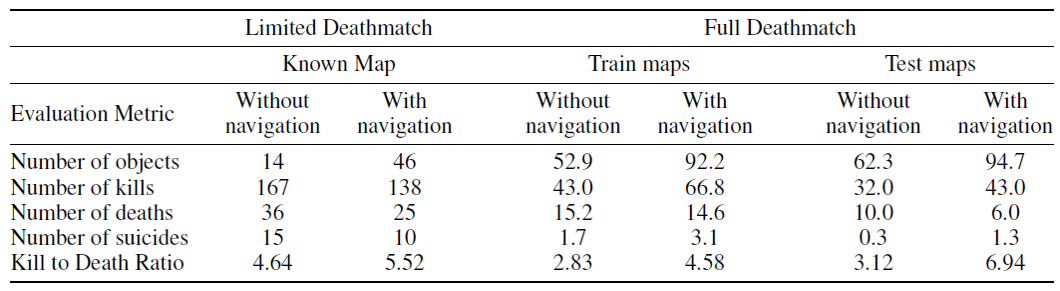
\includegraphics[width=0.9\linewidth]{pictures/fps-exper-result-1}
		\end{figure}
	\end{frame}

	\begin{frame}{实验结果}{Visual Doom AI Competition @ CIG 2016}
		\begin{figure}
			\centering
			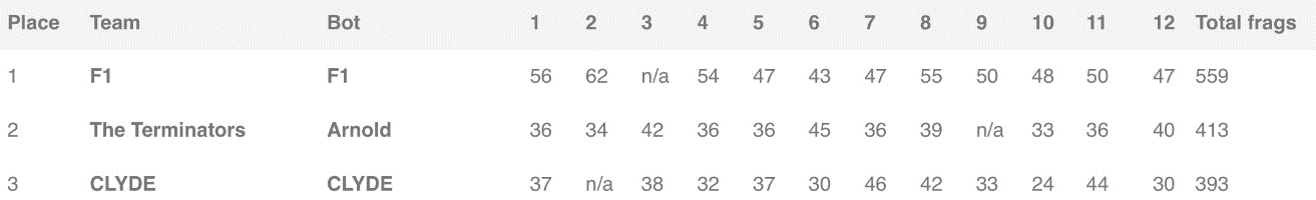
\includegraphics[width=0.9\linewidth]{pictures/fps-exper-result-2}
		\end{figure}
		\begin{figure}
			\centering
			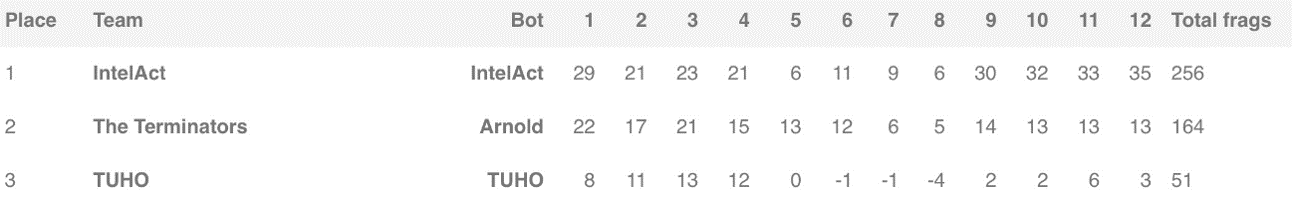
\includegraphics[width=0.9\linewidth]{pictures/fps-exper-result-3}
		\end{figure}
	\end{frame}

	\begin{frame}{实验结果}{Comparison of human players with agent}
		\begin{columns}
			\begin{column}{.5\linewidth}
				\begin{description}
					\item[Single player] 人类和agent分别在独立的游戏中与机器人较量
					
					\item[Multiplayer] 人类与agent相互切磋
					
				\end{description}
			\end{column}
			\begin{column}{.5\linewidth}
				\begin{figure}
					\centering
					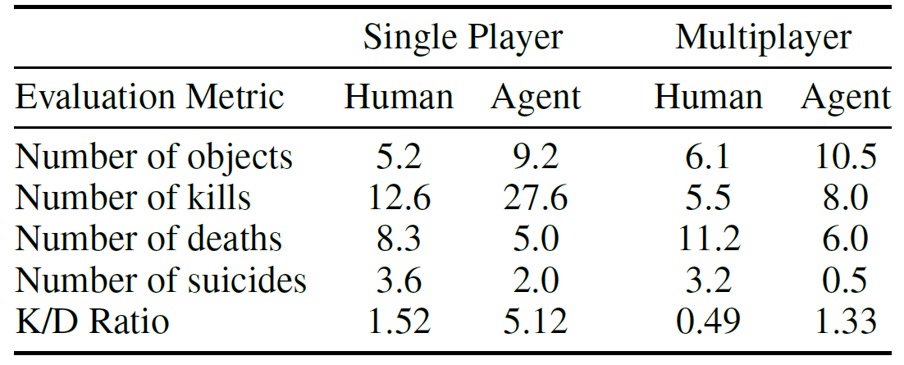
\includegraphics[width=0.9\linewidth]{pictures/fps-exper-result-4}
					\caption{}
					\label{fig:fps-exper-result-4}
				\end{figure}
			\end{column}
		\end{columns}
	\end{frame}

	\begin{frame}{实验结果}{2017 Competition Results}
		\begin{figure}
			\centering
			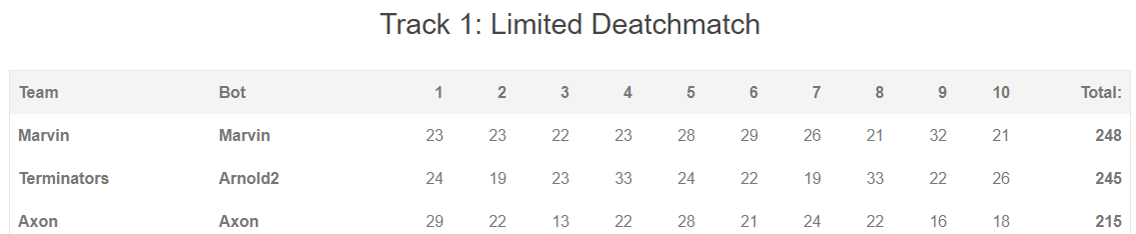
\includegraphics[width=0.9\linewidth]{pictures/fps-exper-result-5}
		\end{figure}
		
		\begin{figure}
			\centering
			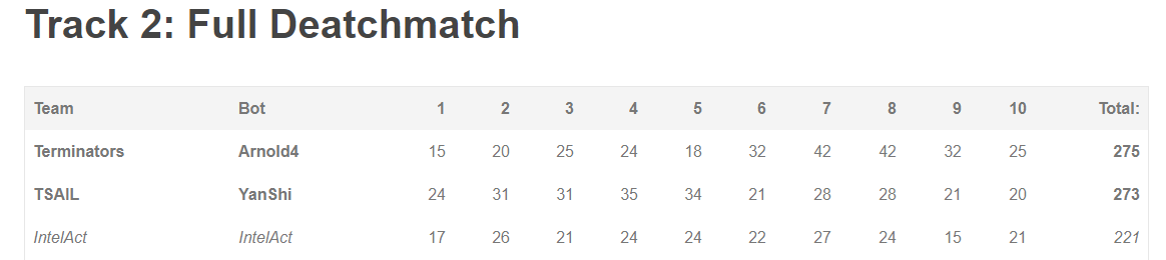
\includegraphics[width=0.9\linewidth]{pictures/fps-exper-result-6}
		\end{figure}
	\end{frame}
		
	\section*{参考文献}
	
	\begin{frame}{参考文献}
		\bibliographystyle{apalike}
		\bibliography{reference}
	\end{frame}
	
	{\background%末页致谢
		\begin{frame}[plain,noframenumbering]
			\finalpage{{\huge 感谢观看!\\ \small Q \& A}}
		\end{frame}
	}
	
\end{document}